%
% File acl2018.tex
%
%% Based on the style files for ACL-2017, with some changes, which were, in turn,
%% Based on the style files for ACL-2015, with some improvements
%%  taken from the NAACL-2016 style
%% Based on the style files for ACL-2014, which were, in turn,
%% based on ACL-2013, ACL-2012, ACL-2011, ACL-2010, ACL-IJCNLP-2009,
%% EACL-2009, IJCNLP-2008...
%% Based on the style files for EACL 2006 by 
%%e.agirre@ehu.es or Sergi.Balari@uab.es
%% and that of ACL 08 by Joakim Nivre and Noah Smith

\documentclass[11pt,a4paper]{article}
\usepackage[hyperref]{acl2018}
\usepackage{times}
\usepackage{latexsym}
\usepackage{graphicx}
\usepackage{url}

%\aclfinalcopy % Uncomment this line for the final submission
%\def\aclpaperid{***} %  Enter the acl Paper ID here

%\setlength\titlebox{5cm}
% You can expand the titlebox if you need extra space
% to show all the authors. Please do not make the titlebox
% smaller than 5cm (the original size); we will check this
% in the camera-ready version and ask you to change it back.

\newcommand\BibTeX{B{\sc ib}\TeX}

\title{Language Understanding Systems --- Mid-Term project: FST \& GRM Tools for SLU}


\author{Claudio Kerov Ghiglianovich \\
  Affiliation / Address line 1 \\
  Affiliation / Address line 2 \\
  Affiliation / Address line 3 \\
  {\tt email@domain} \\\And
  Second Author \\
  Affiliation / Address line 1 \\
  Affiliation / Address line 2 \\
  Affiliation / Address line 3 \\
  {\tt email@domain} \\}

\date{}
 
\begin{document}
\maketitle
\begin{abstract}

\end{abstract}

%\section{Data Analysis}
\section{Data analisys}
\subsection*{Training and testing}
The dataset provided contains the tokenized sentences and specifies the POS-tag related to all the tokens. From that file it was created a lexicon, using the tool \textit{ngramsymbols}, and the corresponding text file in which the sentences are formed only with the IOB-tags. The lexicon included the epsilon and unkown tags, as well as all the IOB-tags. From the two files was created a weighted finite-state machine archive, which is a concatenation of the file representation of one ore more finite-state machines, using the tool \textit{farcompilestrings}. Since one of the objective of the first part was to create a language model, two different tools were used to solve this problem: \textit{ngramcount} and \textit{ngrammake}. The tool \textit{ngramcount} takes as input an archive of FST and gives as output an FST representing the count of the n-grams. The resulting fst is used as input for \textit{ngrammake}, which create a language model. In order to get the most precise language model, ngramcount has a parameter that allows to change the number of token to count, while ngrammake allows to specify which smoothing method for the creation of the final FST. The last objective to complete before starting the testing phase is to create, with \textit{fstcompile}, an FST using the lexicon and the graph matrix representation created at the beginning.
While the first dataset was specific for the training, the second one was for the testing. It has the same format, which is word followed by the corresponding POS-tag. To test the language model and the FST it was necessary to create a different file containing a whole sentence in every row. Every line was transformed into an FST with multiple edges for the same couple of nodes, each of them weighted differently. After being composed with the trained FST and the language model, a shortest path algorithm is applied to the tested FST which results into a final FST with just one edge per couple of nodes. The file with the sentences was used for every type of FST and language model created before. 

\begin{figure}
  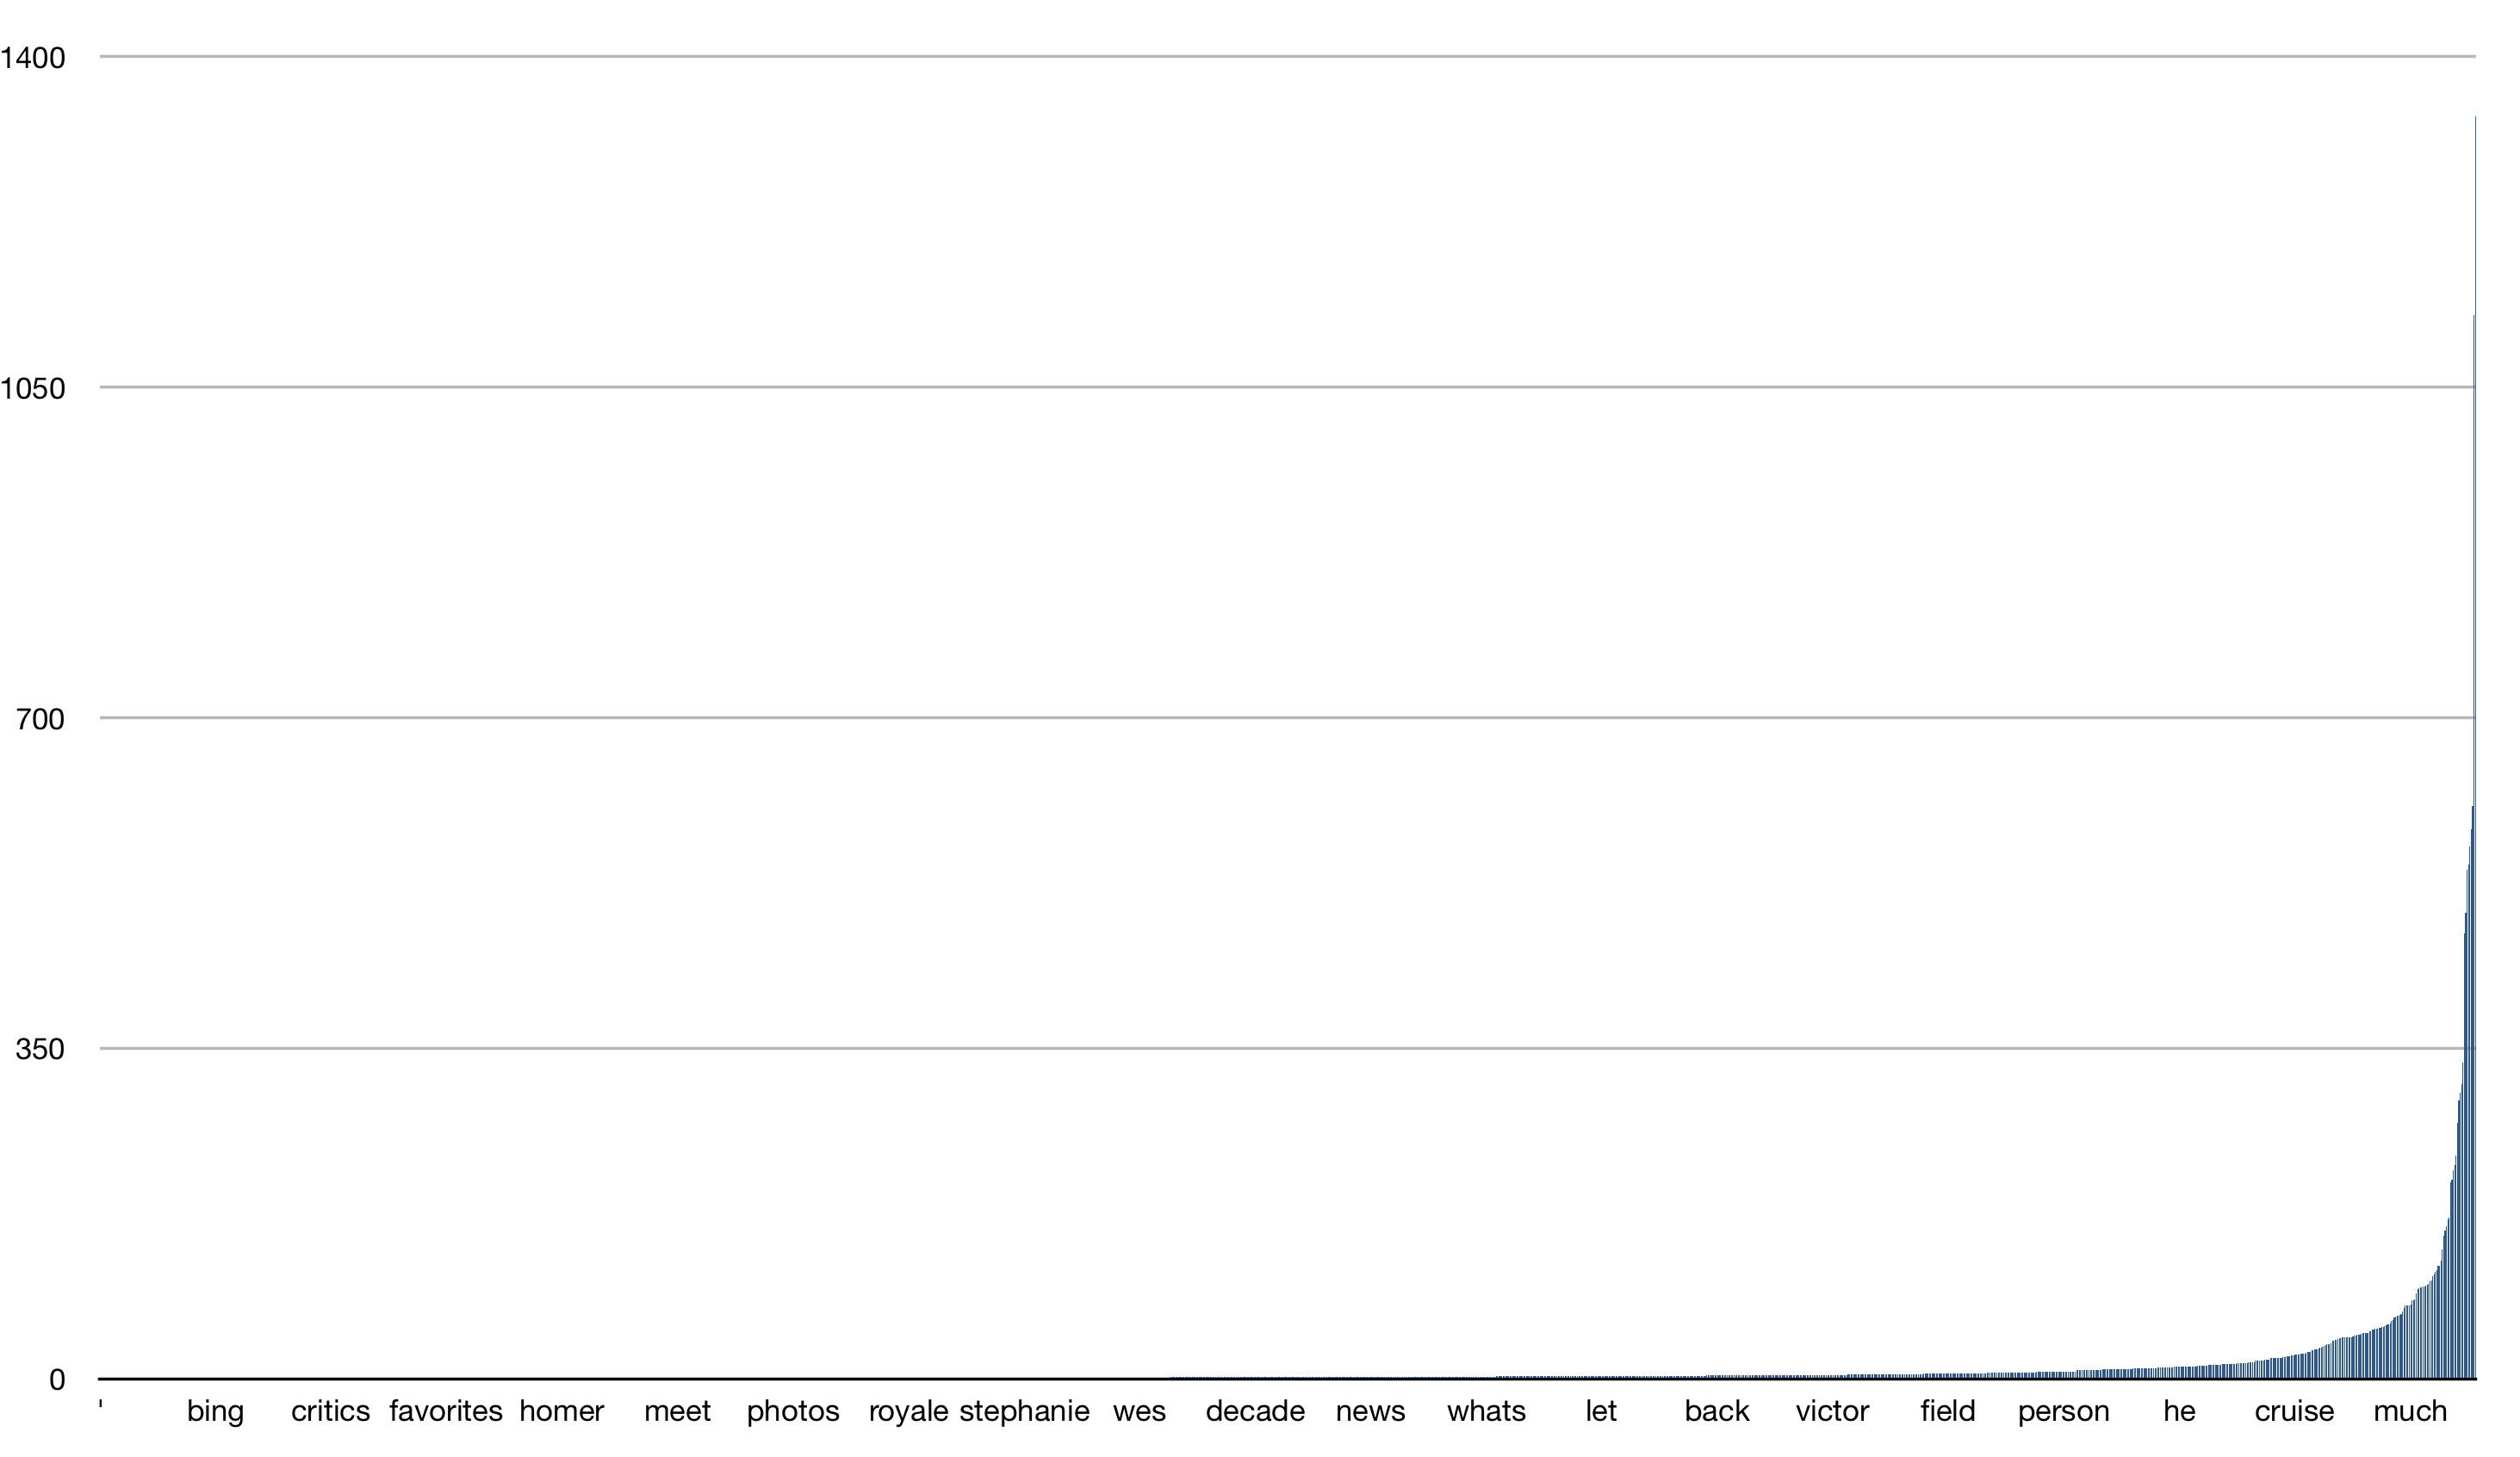
\includegraphics[width=\linewidth]{img/unigram.png}
  \caption{Zipf's law}
  \label{fig:unig}
\end{figure}

\begin{figure}
  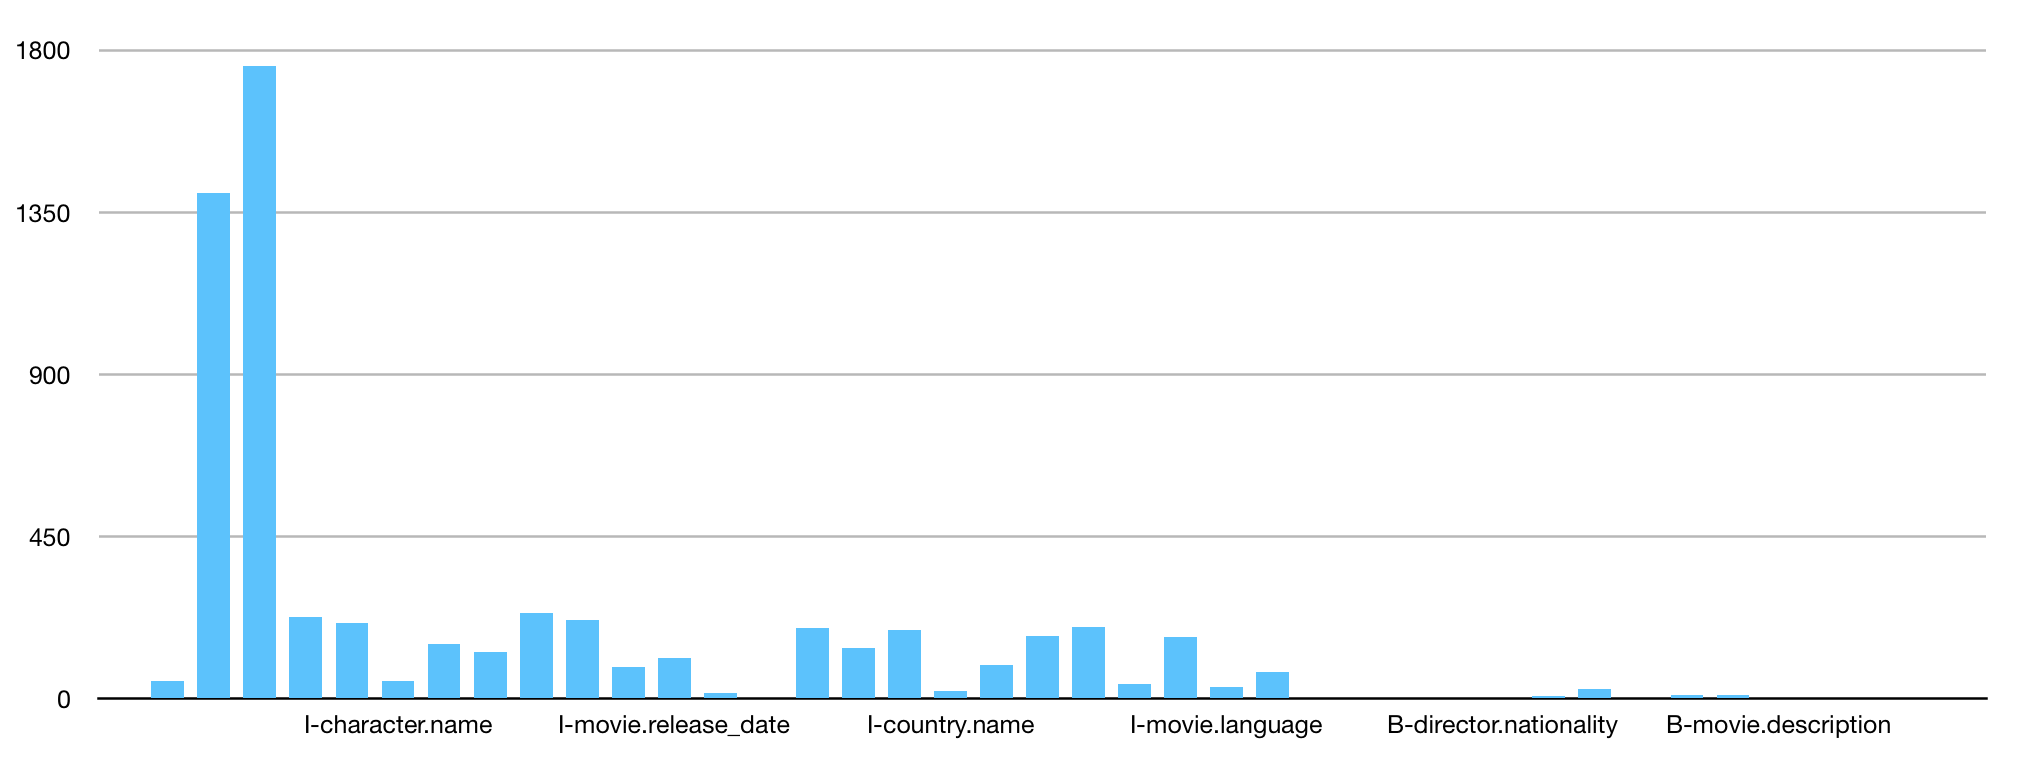
\includegraphics[width=\linewidth]{img/pos.png}
  \caption{POS-tags distribution}
  \label{fig:pos}
\end{figure}

\section{Evaluation}% (with Baseline)}
The evaluation is the last practical phase before the analysis of the reults. There are four tipes of results: true positive, true negative, false positive and false negative. Computing the accuracy is done dividing the summation of the correct decisions by the total amount of instances.
\begin{equation}
Accuracy= \frac{TP + TN} {TP + TN + FP + FN}
\end{equation}
Despite accuracy might seem to be enough, an unknown or infinite value of true negative can lead to a wrong result. Computing precision and recall is a good way to solve this problem.
\begin{equation}
Precision = \frac{TP} {TP + FP}
\end{equation}
\begin{equation}
Recall = \frac{TP}{TP + FN}
\end{equation}
 At this point it is possible to compute the harmonic mean of precision and recall, the F1 score.
 \begin{equation}
F1 =  \frac{2 * Precision * Recall}{Precision + Recall} 
\end{equation}
The output evaluation was made using a perl script called \textit{conlleval}, which takes in input a file containing for every line the token, the real POS-tag and the predicted one, each of them separated by a single space.



\begin{table}[t!]
\begin{center}
\begin{tabular}{|c|c|c|c|c|c|}
\hline
 & 1-gram & 2-gram & 3-gram \\ \hline
Absolute & 57.31 & \textbf{76.31} & 75.62  \\ \hline
Katz & 57.31 & 75.84 & 74.05 \\ \hline
Kneser-Ney & 57.31 & \textbf{76.27} & 75.67 \\ \hline
Unsmoothed & 57.31 & \textbf{76.15} & 75.46 \\ \hline
Presmoothed & 57.31 & \textbf{76.21} & 67.95 \\ \hline
Witten Bell & 57.31 & \textbf{76.31} & 75.52 \\ \hline
\end{tabular}
\caption{F1 Scores for every method and n-grams from 1 to 3}
\label{f1-scores1}
\end{center}
\end{table}


\begin{table}[t!]
\begin{center}
\begin{tabular}{|c|c|c|c|c|c|}
\hline
& 4-gram & 5-gram \\ \hline
Absolute & \textbf{76.04} & \textbf{76.00} \\ \hline
Katz & 73.12 & 63.19 \\ \hline
Kneser-Ney & \textbf{76.04} & \textbf{76.01} \\ \hline
Unsmoothed & 75.85 & 75.90 \\ \hline
Presmoothed & 67.01 & 66.75 \\ \hline
Witten Bell & \textbf{76.07} & \textbf{76.17} \\ \hline
\end{tabular}
\caption{F1 Scores for every method and n-gram 4 and 5}
\label{f1-scores2}
\end{center}
\end{table}

 The baseline F1 score is 57.31 for all methods, as showed on table \ref{f1-scores1}, while the best performances were obtained with 2-grams and the method ``absolute`` and ``Witten Bell``.
\section{Discussion}



\end{document}
